% !TeX root = main.tex
% Edit by: CamuseCao

\chapter{随机变量及其分布}

为了进行定量的数学处理,必须把随机现象的结果数量化.这就是引进随机变量的原因随机变量的引进使得对随机现象的处理更简单与直接,也更统一而有力.本章我们将主要讨论一维随机变量及其分布.

\section{随机变量及来分布}

在第一章中我们曾提及随机变量,在那里我们把“用来表示随机现象结果的变量“称为随机变量,其中“表示”一词的含义是什么?这是要进一步探讨的问题.

\subsection{随机变量的概念}

在随机现象中有很多样本点本身就是用数量表示的,由于样本点出现的随机性,其数量呈现为随机变量,譬如

\begin{itemize}
	\item 掷一颗散子,出现的点数X是一个随机变量.
	\item 每天进入某超市的顾客数Y;顾客购买商品的件数 $U$ ;顾客排队等候付款的时间 $V,Y,LU,V$ 是三个不同的随机变量,
	\item 电视机的寿命T是一个随机变量.·测量的误差.是一个随机变量.
	\item 测量的误差 $\epsilon $ 是一个随机变量.
\end{itemize}

在随机现象中还有不少样本点本身不是数,这时可根据研究需要设计随机变量,譬如
\begin{itemize}
	\item 检查一个产品,只考察其合格与否,则其样本空间为Q=|合格品,不合格品,这时可设计一个随机变量 $X$ 如下:
\end{itemize}

\begin{table}[htbp]
	\centering
	\begin{tabular}{ccc}
		样本点   &       & X的取值 \\\hline
		合格品   &   $ \longrightarrow $ & 0 \\
		不合格品 &    $ \longrightarrow $ & 1 \\
	\end{tabular}%
\end{table}%

在此可将 $ X $ 解释为“检查一个产品中不合格品数”.若此种产品的不合格品率为$ p $,则$ X $取各种值的概率可列表如下:

\begin{table}[htbp]
	\centering
	\begin{tabular}{c|cc}
		$ X $     & $ 0 $     & $ 1 $ \\\hline
		$ P $     & $ 1-p $   & $ p $ \\
	\end{tabular}%
\end{table}%


\begin{itemize}
	\item 检查三个产品,则有8个样本点,若记X为“三个产品中的不合格品数”,则$ X $与样本点之间有如下对应关系:
\end{itemize}

\begin{table}[htbp]
	\centering
	\begin{tabular}{ccc}
		样本点   &       & $ X $的取值 \\\hline
		$ \omega_1=(0,0,0) $ &   $ \longrightarrow $    & 0 \\
		$ \omega_2=(1,0,0) $ &   $ \longrightarrow $    & 1 \\
		$ \omega_3=(0,1,0) $ &   $ \longrightarrow $    & 1 \\
		$ \omega_4=(0,0,1) $ &   $ \longrightarrow $    & 1 \\
		$ \omega_5=(0,1,1) $ &   $ \longrightarrow $    & 2 \\
		$ \omega_6=(1,0,1) $ &   $ \longrightarrow $    & 2 \\
		$ \omega_7=(1,1,0) $ &   $ \longrightarrow $    & 2 \\
		$ \omega_8=(1,1,1) $ &   $ \longrightarrow $    & 3 \\
	\end{tabular}%
\end{table}%

这样$ X $取各种值就是如下的互不相容的事件:

\begin{equation} 
\begin{array}{ll}
{ \{ X=0 \}=\{\omega_{1}\} ;} & \{  X=1 \}=\{\omega_{2}, \omega_{3}, \omega_{4} \} \\ 
{ \{ X=2 \}=\{\omega_{5}, \omega_{6}, \omega_{7}\}}\quad &{\{ X=3\}=\{ \omega_{8} \}}
\end{array}
\end{equation}

若此种产品的不合格品率为$ p $,则$ X $取各种值的概率可列表如下:

\[ 
\begin{array}{c|cccc}{x} & {0} & {1} & {2} & {3} \\ \hline P & {(1-p)^{3}} & {3 p(1-p)^{2}} & {3 p^{2}(1-p)} & {p^{3}}\end{array}
\]

\begin{definition}
	定义在样本空间$ Q $上的实值函数$ X=X(\omega) $称为随机变量,常用大写字母$ X,Y,Z $等表示随机变量,其取值用小写字母$ x,y,x $等表示.假如一个随机变量仅取有限个或可列个值,则称其为离散随机变量.假如一个随机变量的可能取值充满数轴上的一个区间$ (a,b) $,则称其为连续随机变量,其中$ a $可以是$ -\infty ,b $可以是$ +\infty $.
\end{definition}


这个定义表明:随机变量$ X $是样本点$ \omega $的一个函数,这个函数可以是不同样本点对应不同的实数,也允许多个样本点对应同一个实数.这个函数的自变量(样本点)可以是数,也可以不是数,但因变量一定是实数.

与微积分中的变量不同,概率论中的随机变量$ X $是一种“随机取值的变量”.以认识离散随机变例,我们不仅要知道$ Y $取哪些值,而且还要知道它取这些值的概率各是多少,这就需要分布的概念.有没有分布是区分一般变量与随机变量的子要标志.

\subsection{随机变量的分布函数}

随机变量$ X $是样个点$ \omega $的一个值函数.若$ B $是某些实数组成的集合,即$ B\subset R $,$ R $表小实数集、则$ X\subset B $表示如下的随机事件

\[
\omega X(\omega)\subset B \subset \Omega
\]

这就是我们可以用随性变立量得某些取值来表示随机事件的依据.臂如

\begin{itemize}
	\item 记$ X $表示掷一颗骰子出现的点数,明$ X $的可能取值为$ 1,2\dotsc ,6 $.这是一个离散随机变量.事件A“点数小于等等于3”,可以表示为$ A=\{X\leq 3\} $.
	\item 记$ Y $表示一天内到达某商场得顾客数.则$ Y $的可能取值为$ 0,1,2\dotsc ,n\dotsc $这也是一个离散随机变量.事件B“至少来1000位顾客”,可以表示为$ B=\{ X\geq 1000 \} $.
	\item 记$ T $表示某电器品的使目寿命,则T的可能取值充满区间$ [0,+o\infty ) $.这楚一个连续随机变量.事件C“使用寿命在40000至50000小时之间”,可以表示为$ C=\{ 40000 \leq 50000 T\} $ . 
\end{itemize}



为了掌握$ X $的统计规律性,我们只要掌握$ X $取各种值的概率.由于

\[
\{a < X \leq b \} = \{ X \leq b\} - \{x\leq a\},
\]

因此只要对任意实数$ x $,知道了件$ X\geq x $的概率就够了,这个概率具有累积特性,常用$ F $表示.另外这个概率与$ x $有关,不同的$ x $,此累积概率的值也不同,为此记

\[
F(X,P(X\leq x))
\]

于是$ F(x) $所有$ x $都有定义,而$ F(x) $是定义在$ (\infty,+\infty ) $上、取值于$ [0,1] $的一个函数.这就是我们下面要引入的分布函数.

\begin{definition}{}{}
	设$ X $是一个随机变量,对任意实数$ x $,称
	\begin{equation} 
	F(x)=P(X \leqslant x) \label{2.1.1}
	\end{equation}
	为随机变量$ X $的分布函数.且称$ X $服从$ F(x) $,记为$ X\sim F(x) $.有时也可用$F_{X}(x)$以表明是$ X $的分布函数(把$ X $作为$ F $的下标).
\end{definition}

\begin{example}
	向半径为$ r $的圆内随机抛一点,求此点到圆心之距离$ X $的分布函数$ F(x) $,并求$P\left(X>\frac{2 r}{3}\right)$.
	
	解事件“$ x=x $”表示所抛之点落在半径为$x(0 \leqslant x \leqslant r)$的圆内,故由几何概率知
	
	\[ 
	F(x)=P(X \leqslant x)=\frac{\pi x^{2}}{\pi r^{2}}=\left(\frac{x}{r}\right)^{2}
	\]
	
	从而
	
	\[ 
	P\left(X>\frac{2 r}{3}\right)=1-P\left(X \leqslant \frac{2 r}{3}\right)=1-\left(\frac{2}{3}\right)^{2}=\frac{5}{9}
	\]
	
	
\end{example}


从分布函数的定义可见,任一随机变量$ X $(离散的或连续的)都有一个分布函数.有了分布函数,就可据此算得与随机变量$ X $有关事件的概率.下面先证明分布函数的三个基本性质.

\begin{theorem}
	任一分布函数F(x)都具有如下三条基本性质:
	\begin{enumerate}
		\item \textbf{单调性} $ F(x) $是定义在整个实数轴$ (-\infty,+\infty ) $上的单调非减函数,即对任意的$ x_1<x_2 $,有$ F(x_1)\leq F(x_2) $.
		\item 有界性对任意的$ x $,有$ 0\leq F(x)\leq 1 $,且
		\[ 
		\begin{array}{l}{F(-\infty)=\lim _{x \rightarrow-\infty} F(x)=0} \\ {F(+\infty)=\lim _{x \rightarrow+\infty} F(x)=1}\end{array}
		\]
		
		\item 右连续性$ F(x) $是$ x $的右连续函数,即对任意的$ x_0 $,有
		\[ 
		\lim _{x \rightarrow x_{0}+} F(x)=F\left(x_{0}\right)
		\],
		即
		\[ 
		F\left(x_{0}+0\right)=F\left(x_{0}\right)
		\]
	\end{enumerate}
\end{theorem}

\begin{proof}
	(1)是显然的,下证(2).由于$ F(x) $是事件$\{X \leqslant x\}$的概率,所以$ 0\leq 
	F(x)\leq 1 $.由$ F(x) $的单调性知,对任意整数$ m $和$ n $,有
	
	\[ 
	\lim _{x \rightarrow-\infty} F(x)=\lim _{m \rightarrow-\infty} F(m), \lim _{x \rightarrow+\infty} F(x)=\lim _{n \rightarrow+\infty} F(n)
	\]
	
	都存在.又由概率的可列可加性得
	
	\[ 
	\begin{array}{ll}
	1=P(-\infty<X<+\infty)&=P\left(\bigcup_{i=-\infty}^{+\infty}\{i-1<X \leqslant i\}\right) \\ &=\sum_{i=-\infty}^{+\infty} P(i-1<X \leqslant i)=\lim _{n \rightarrow+\infty \atop n \rightarrow+\infty} \sum_{m \rightarrow+\infty}^{n} P(i-1<X \leqslant i) \\ &=\lim _{n \rightarrow+\infty} F(n)-\lim _{m \rightarrow-\infty} F(m)
	\end{array}
	\]
	
	再证(3),因为$ F(x) $是单调有界非降函数,所以其任一点$ x_0 $的右极限$ F(x_0+0) $必存在.为证右连续性,只要对单调下降的数列$x_{1}>x_{2}>\cdots>x_{n}>\cdots>x_{0}$,当$x_{n} \rightarrow x_{0}(n \rightarrow+\infty)$时,证明$\lim _{n \rightarrow+\infty} F\left(x_{n}\right)=F\left(x_{0}\right)$成立即可.因为
	
	\[ \begin{array}{ll}
	F\left(x_{1}\right)-F\left(x_{0}\right)&=P\left(x_{0}<X \leqslant x_{1}\right)=P\left(\bigcup_{r=1}^{+\infty}\left\{x_{i+1}<X \leqslant x_{i}\right\}\right) \\
	&=\sum_{i=1}^{+\infty} P\left(x_{i+1}<X \leqslant x_{i}\right)=\sum_{i=1}^{+\infty}\left[F\left(x_{i}\right)-F\left(x_{t+1}\right)\right] \\
	&=\lim _{n \rightarrow \infty}\left[F\left(x_{1}\right)-F\left(x_{n}\right)\right]=F\left(x_{1}\right)-\lim _{n \rightarrow \infty} F\left(x_{n}\right)
	\end{array}\]
\end{proof}

由此得

\[ 
F\left(x_{0}\right)=\lim _{x \rightarrow+\infty} F\left(x_{n}\right)=F\left(x_{0}+0\right)
\]

至此三条基本性质全部证得.

以上三条基本性质是分布函数必须具有的性质,还可以证明:满足这三个基本性质的函数一定是某个随机变量的分布函数.从而这三个基本性质成为判别某个函数是否能成为分布函数的充要条件.

有了随机变量$ X $的分布函数,那么有关$ X $的各种事件的概率都能方便地用分布函数来表示了,例如,对任意的实数$ a $与$ b $,有

\[ 
\begin{array}{ll}
P(a<X \leqslant b)&=F(b)-F(a)\\ 
P(X=a)&=F(a)-F(a-0) \\
P(X \geqslant b)&=1-F(b-0)\\
P(X>b)&=1-F(b)\\ 
P(a<x<b)&=F(b-0)-F(a)\\
P(a \leqslant X \leqslant b)&=F(b)-F(a-0)\\ 
P(a \leqslant X<b)&=F(b-0)-F(a-0)
\end{array}
\]

特别当$ F(x) $在$ a $与$ b $处连续时,有

\[ 
F(a-0)=F\langle a), \quad F(b-0)=F(b)
\]

这些公式将会在今后的概率计算中经常遇到.

\begin{example}
	设有一反正切函数
	\[ 
	F(x)=\frac{1}{\pi}\left[\arctan x+\frac{\pi}{2}\right], \quad-\infty<x<+\infty
	\]
	
	它在整个数轴上是连续、单调严增函数,且$F(+\infty)=1, F(-\infty)=0$.由于此$ F(x) $满足分布函数的三个基本性质,故$ F(x) $是一个分布函数.称这个分布函数为柯西分布函数,其图形见图~\ref{fig:2-1-1}
	
	\begin{figure}
		\centering
		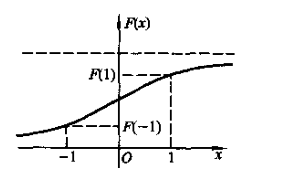
\includegraphics[width=0.7\linewidth]{2-1-1}
		\caption{柯西分布函数}
		\label{fig:2-1-1}
	\end{figure}
	
	若X服从柯西分布,则
	
	\[ 
	\begin{aligned} P(-1 \leqslant X \leqslant 1) &=F(1)-F(-1) \\ &=\frac{1}{\pi}[\arctan (1)-\arctan (-1)] \\ &=\frac{1}{\pi}\left[\frac{\pi}{4}-\left(-\frac{\pi}{4}\right)\right]=\frac{1}{2} \end{aligned}
	\]
	
\end{example}

\subsection{高散随机变量的概率分布列}

对离散随机变量而言,常用以下定义的分布列来表示其分布.

\begin{definition}{}{}
	设$ X $是一个离散随机变量,如果$ X $的所有可能取值是$ x_1,x_{2}, \cdots, x_{n}, \cdots$ 则称$ X $取$ x_i $, 的概率
	\begin{equation} 
	p_{i}=p\left(x_{i}\right)=P\left(X=x_{i}\right), i=1,2, \cdots, n, \cdots \label{eq:2.1.2}
	\end{equation}
	
	为$ X $的概率分布列或简称为分布列,记为$X \sim\left|p_{t}\right|$,分布列也可用如下列表方式来表示:
	
	\[
	\begin{array}{c|ccccc}
	X	&    x_{1}     &    x_{2}     &    \cdots     &     x_{n}    &   \cdots \\
	P	&    p(x_1)     &    p(x_2)     &    \cdots     &    p(x_n)     &   \cdots \\
	\end{array}
	\]
	
	
	或记成
	
	\[ 
	\left( \begin{array}{ccccc}{x_{1}} & {x_{2}} & {\cdots} & {x_{n}} & {\cdots} \\ {p\left(x_{1}\right)} & {p\left(x_{2}\right)} & {\cdots} & {p\left(x_{n}\right)} & {\cdots}\end{array}\right]
	\]
	
\end{definition}


第一章中我们已见过多个分布列,不同的离散随机变量可能有不同的分布列,甚至在一个样本空间上可以定义几个服从不同分布列的随机变量,这要看我们的研究需要,下面就是在同一样本空间上给出几个不同随机变量的具体例子.
\begin{example}
	掷两颗骰子,其样本空间O含有36个等可能的样本点
	
	\[ 
	\Omega=\{(x, y) ; x, y=1,2, \cdots, 6\}
	\]
	在$ \Omega $上定义如下3个随机变量$ X,Y $和$ Z $:
	\begin{itemize}
		\item $ X $为点数之和,其可能取值为$2,3, \cdots, 12$等共11个值,其定义见~\ref{fig:2-1-2}(a)
		\item $ Y $为6点的个数,其可能取值为$ 0,1,2 $等共$ 3 $个值,其定义见图~\ref{fig:2-1-2}(b).
		\item $ Z $为最大点数,其可能取值为$1,2, \cdots, 6$等共$ 6 $个值,其定义见图~\ref{fig:2-1-2}(c)
	\end{itemize}
\end{example}


\begin{figure}
	\centering
	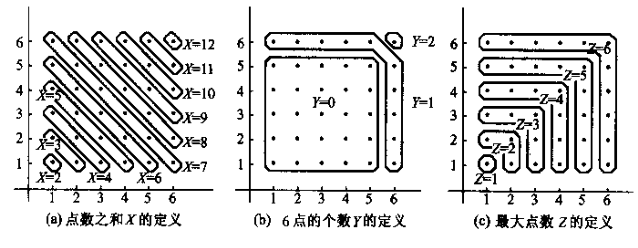
\includegraphics[width=0.7\linewidth]{2-1-2}
	\caption{同一样本空间上不同随机变量}
	\label{fig:2-1-2}
\end{figure}

这三个随机变量的分布列可用古典方法算得如下:
·.
% Table generated by Excel2LaTeX from sheet '1'
\begin{table}[htbp]
	\centering
	\begin{tabular}{c|cccccrrrrrr}
		X     & 2     & 3     & 4     & 5     & 6     & \multicolumn{1}{c}{7} & \multicolumn{1}{c}{8} & \multicolumn{1}{c}{9} & \multicolumn{1}{c}{10} & \multicolumn{1}{c}{11} & \multicolumn{1}{c}{12} \\\hline
		P     &   $ \frac{1}{36} $    &   $ \frac{2}{36} $    &   $ \frac{3}{36} $    &   $ \frac{4}{36} $    &    $ \frac{5}{36} $   &   $ \frac{6}{36} $    &   $ \frac{5}{36} $    &    $ \frac{4}{36} $   &    $ \frac{3}{36} $   &    $ \frac{2}{36} $   &  $ \frac{1}{36} $\\
	\end{tabular}%
	
	\begin{tabular}{c|ccc}
		$ Y $     & 0     & 1     & 2 \\\hline
		$ P $     &  $ \frac{25}{36} $     &    $ \frac{10}{36} $   & $ \frac{1}{36} $ \\
	\end{tabular}%
	
	\begin{tabular}{c|rccccc}
		$ Z $     & 1 & 2     & 3     & 4     & 5     & 6 \\\hline
		$ P $     &   $ \frac{1}{36} $    &   $ \frac{3}{36} $    &   $ \frac{5}{36} $    &   $ \frac{7}{36} $    &   $ \frac{9}{36} $    &  $ \frac{11}{36} $\\
	\end{tabular}%
\end{table}%


类似地,还可以在这个样本空间上定义其他的离散随机变量.

分布列的基本性质


(1)非负性:$: p\left(x_{t}\right) \geqslant 0, i=1,2, \cdots$;
(2)正则性:$\sum_{i=1}^{\infty} p\left(x_{i}\right)=1$.

以上两条基本性质是分布列必须具有的性质,也是判别某个数列是否成为分布列的充要条件
由离散随机变量X的分布列很容易写出X的分布函数:

\[ 
F(x)=\sum_{x_{1} \leqslant x} p\left(x_{i}\right)
\]

它的图形是有限级(成无穷级)的阶梯函数,具体见下面的例子.不过在离散场合,常用来描述其分布的是分布列,很少用到分布函数.因为求离散随机变量X的有关事件的概率时,用分布列比用分布函数来得更方便.

\begin{example}
	设离散随机变量$ X $的分布列为
	
	\[ 
	\begin{array}{c|ccc}
	x & -1 & 2 & 3 \\\hline
	P & 0.25 & 0.5 & 0.25 \\
	\end{array}
	\]
	
	试求$P(X \leqslant 0.5), P(1.5<X \leqslant 2.5)$,并写出$ X $的分布函数.
	
	\textbf{解}
	
	\[ 
	\begin{array}{l}{P(X \leqslant 0.5)=P(X=-1)=0.25} \\ {P(1.5<X \leqslant 2.5)=P(X=2)=0.5}\end{array}
	\]
	
	\[ 
	F(x)=\left\{\begin{array}{ll}
	{0,} & {x<-1} \\ 
	{0.25,} & {-1 \leqslant x<2} \\ 
	{0.25+0.5=0.75,} & {2 \leqslant x<3} \\ 
	{0.25+0.5+0.25=1,} & {x \geqslant 3}
	\end{array}\right.\]
	
	$ F(x) $的图形如图~\ref{fig:2-1-3}所示,它是一条阶梯形的曲线,在$ X $的可能取值$-1,2,3$处有跳跃点,其跳跃度分别为$ 0.25,0.5,0.25 $ .
	
	
	特别,常量$ c $可看作仅取一个值的随机变量X,即
	
	\begin{figure}
		\centering
		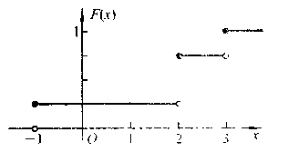
\includegraphics[width=0.7\linewidth]{2-1-3}
		\caption{离散随机变量的分布雨数}
		\label{fig:2-1-3}
	\end{figure}
	
	\[ 
	P(X=c)=1
	\]
	
	这个分布常称为单点分布或退化分布,它的分布函数是
	
	\begin{equation}
	F(x)=\left\{\begin{array}{ll}
	{0,} & {x<c} \\ 
	{1,} & {x \geqslant c}
	\end{array}\right.  \label{eq:2.1.3}
	\end{equation}
	
	其图形为
	\begin{figure}
		\centering
		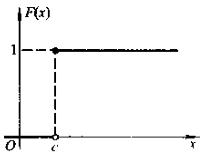
\includegraphics[width=0.7\linewidth]{2-1-4}
		\caption{单点分布函数}
		\label{fig:2-1-4}
	\end{figure}
	
	
\end{example}

以下例子说明:在具体求离散随机变量$ X $的分布列时,关键是求出$ X $的所有可能取值及取这些值的概率.

\begin{example}
	一汽车沿一街道行驶,需要经过3个设有红绿信号灯的路口,若设每个信号灯显示红绿两种信号的时间相等,且各个估号灯l.作相互独立.以x表示该汽车首次遇到红灯前已通过的路口数.试求$ X $的概率分布列.
	
	解由题设可知,$ X $的可能取值为$ 0,1.2.3 $又记$ A= $“汽车在第i个路口遇到红灯”,$ i=1,2,3 $.因为$ A_1,A_2,A_3 $相互独立,且
	
	\[ 
	P\left(A_{t}\right)=P\left(A_{t}\right)=\frac{1}{2}, \quad i=1.2 .3
	\]
	所以得
	
	\[ 
	\begin{array}{l}
	{P(X=0)=P\left(A_{1}\right)=\frac{1}{2}} \\ 
	{P(X=1)=P\left(\overline{A}_{1} A_{2}\right)=P\left(\overline{A}_{1}\right) P\left(\Lambda_{2}\right)=\frac{1}{4}} \\ 
	{P(X=2)=P\left(\overline{A}_{1} \overline{A}_{2} A_{3}\right)=P\left(A_{1}\right) P\left(\dot{A}_{2}\right) P\left(A_{J}\right)=\frac{1}{8}}\\
	{P(X=3)=P\left(\overline{A}_{1} \overline{A}_{2} \overline{A}_{3}\right)=P\left(\overline{A}_{1}\right) P\left(\overline{A}_{2}\right) P\left(\overline{A}_{2}\right)=\frac{1}{8}}
	\end{array}
	\]
	
	故$ X $的分布列如下:
	
	% Table generated by Excel2LaTeX from sheet '1'
	\begin{table}[htbp]
		\centering
		\begin{tabular}{c|cccc}
			$ X $     & 0     & 1     & 2     & 3 \\\hline
			$ P $     & 1/2   & 1/4   & 1/8   & 1/8 \\
		\end{tabular}%
	\end{table}%
	
\end{example}

\subsection{连续随机变量的概率密度函数}

连续随机变量的一切可能取值是充满某个区间$ (a,b) $,在这个区间内有无穷不可列个实数,因此描述连续随机变量的概率分布不能再用分布列形式表示,而要改用概率密度函数表示.下面用一个实例来导出概率密度函数的由来.

\begin{example}
	新生婴儿的体重X是一个随机变量.假如记录很多个(例如:十万个)新生婴儿的体重,我们将各种体重的频率用直方图形式表示出来,x轴表示体重(单位:$ 500g $),$ y $轴表示单位长度上的频率,则以下图~\ref{fig:2-1-5}的(a)至(c)
	表明:当$\Delta x=1$越来越小,其频率直方图形越来越光滑.
	
	\begin{enumerate}
		\item 当$\Delta x=1$ ,体重的频率直方图见图~\ref{fig:2-1-5}(a).注意,图中矩形宽度为1,高度为频率,所以所有矩形面积之和为1.此时体重$ X $的取值为$1,2, \cdots $即$ X $是一个离散随机变量.
		\item 当 $\Delta x=0.1$ ,体重的频率直方图见图~\ref{fig:2-1-5}(b).注意,图中矩形宽度为
		$ 0.1 $,高度为:频率$ /0.1 $,所有小矩形面积之和仍为1.
		\item 当 $\Delta x \rightarrow 0$ 则体重的频率图趋于图~\ref{fig:2-1-5}(c)所示的一条光滑的曲线,其高度为概率密度值.如果记这条曲线为$ p(x) $,则$ p(x) $与$ x $轴所夹面积仍为1.此时体重$ X $的取值充满了某一区间,即X是一个连续随机变量.图中$ p(x) $就是连续随机变量X的概率密度函数.
	\end{enumerate}
	
\end{example}

\begin{figure}
	\centering
	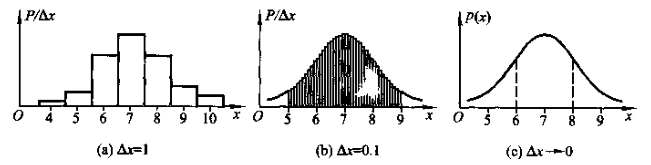
\includegraphics[width=0.7\linewidth]{2-1-5}
	\caption{新生婴儿体重$ X $的频率分布}
	\label{fig:2-1-5}
\end{figure}

下面给出连续随机变量的概率密度函数的定义.

\begin{definition}
	设随机变量$ X $的分布函数为$ F(x) $,如果存在实数轴上的一个非负可积函数$ p(x) $,使得对任意实数$ x $有
	\begin{equation} 
	F(x)=\int_{-\infty}^{x} p(t) \mathrm{d} t \label{eq:2.1.4}
	\end{equation}
	
	从~\ref{eq:2.1.4}式可以看出,在$ F(x) $导数存在的点上有
	\begin{equation} 
	F^{\prime}(x)=p(x) \label{eq:2.1.5}
	\end{equation}
	
	$ F(x) $是(累积)概率函数,其导数$ F'(x) $是概率密度函数,由此可看出$ p(x) $被称为概率密度函数的理由.
	
	由~\ref{eq:2.1.5}式,可从分布函数求得密度函数.譬如例2.1.2给出的柯西分布函数处处可导,故柯西分布的密度函数为
	
	\[ 
	p(x)=\frac{1}{\pi} \frac{1}{1+x^{2}},-\infty<x<+\infty
	\]
\end{definition}

$ 密度函数的基本性质 $

(1)非负性:$p(x) \geqslant 0$;

(2)正则性:$: \int_{-\infty}^{+\infty} p(x) \mathrm{d} x=1$.

以上两条基本性质是密度函数必须具有的性质,也是确定或判别某个函数是否成为密度函数的充要条件.譬如已知某个函数$ p(x) $为密度函数,若$ p(x) $中有待定常数,则该常数必定是利用正则性$\int_{-\infty}^{+\infty} p(x) \mathrm{d} x=1$来确定的,见下面例子.

\begin{example}
	已知随机变量X的密度函数为
	
	\[ 
	p(x)=\left\{\begin{array}{ll}
	{c,-1 \leqslant x \leqslant 1} \\ 
	{0,\text{其它}}
	\end{array}\right.
	\]
	
	试求常数$ c $.
	
	\textbf{解} 由密度函数的正则性知
	
	\[ 
	1=\int_{-\infty}^{+\infty} p(x) \mathrm{d} x=\int_{-1}^{1} c \mathrm{d} x=2 c
	\]
	
	所以由$ 2c=1 $得$ c=0.5 $.利用分段积分,我们还可求出$ X $的分布函数.
	
	当$ x<-1 $时,
	\[ 
	F(x)=\int_{-\infty}^{x} 0 \mathrm{d} t=0
	\]
	
	当$-1 \leqslant x<1$时,
	\[ 
	F(x)=\int_{-3}^{x} 0.5 \mathrm{d} t=(x+1) / 2
	\]
	
	当 $x \geqslant 1$ 时,
	\[ 
	F(x)=\int_{1}^{1} 0.5 \mathrm{d} t+\int_{1}^{x} 0 \mathrm{d} t=1
	\]
	
	所以得$ X $的分布函数为
	
	\[ 
	F(x)=\left\{\begin{array}{ll}
	{0,} & {x<-1} \\ 
	{\frac{x+1}{2},} & {-1 \leqslant x<1} \\ 
	{1,} & {x \geqslant 1}
	\end{array}\right.
	\]
	
\end{example}


由密度函数求分布函数的关键是;分布函数是一种“累积”概率,所以在计算积分时要注意积分限的合理运用.此例密度函数和分布函数的图形如图2.1.6
(a)与(b)所示,这个分布称为区间(-1,1)上的均匀分布,记为U(-1,1).

\begin{figure}
	\centering
	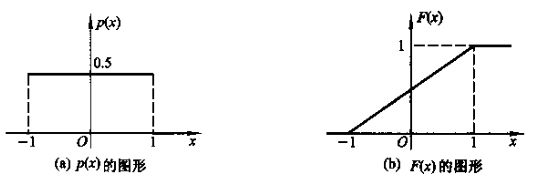
\includegraphics[width=0.7\linewidth]{2-1-6}
	\caption{均匀分布$U(-1,1)$的密度函数和分布函数的图形}
	\label{fig:2-1-6}
\end{figure}

\begin{example}
	设随机变量X的密度函数为
	
	\[ 
	p(x)=\left\{\begin{array}{ll}{x,} & {0 \leqslant x<1} \\ {2-x,} & {1 \leqslant x<2} \\ {0,} & {\text{其它}}\end{array}\right.
	\]
	
	试求$ X $的分布函数$ F(x) $.
	
	\textbf{解} 当$ x<0 $时,
	\[ 
	F(x)=\int_{-\infty}^{x} p(x) \mathrm{d} x=0
	\]
	
	当 $0 \leqslant x<1$ 时,
	\[ 
	F(x)=\int_{0}^{x} x \mathrm{d} x=\frac{x^{2}}{2}
	\]
	
	当 $1 \leqslant x<2$时,
	\[ 
	F(x)=\int_{-\infty}^{x} p(x) \mathrm{d} x=\int_{0}^{1} x \mathrm{d} x+\int_{1}^{x}(2-x) \mathrm{d} x=-\frac{x^{2}}{2}+2 x-1
	\]
	
	当 $\mathrm{I} \leqslant x<2$ 时,
	\[ 
	F(x)=\int_{-\infty}^{x} p(x) \mathrm{d} x=\int_{0}^{1} x \mathrm{d} x+\int_{1}^{2}(2-x) \mathrm{d} x=1
	\]
	
	综上所述,得$ X $的分布函数为
	
	\[ 
	F(x)=\left\{\begin{array}{ll}
	{0,} & {x<0} \\ 
	{\frac{x^{2}}{2},} & {0 \leqslant x<1} \\ 
	{-\frac{x^{2}}{2}+2 x-1,} & {1 \leqslant x<2} \\ 
	{1,} & {x \geqslant 2}
	\end{array}\right.
	\]
\end{example}

这个分布被称为辛普森分布或三角分布,其密度函数$ p(x) $和分布函数$ F(x) $的图形见下图~\ref{fig:2-1-7}.从图形上可看出:在区间$ (0,1) $上$ F(x) $是下凸函数,在区间$ (1,2) $上$ F(x) $是上凸函数.

\begin{figure}
	\centering
	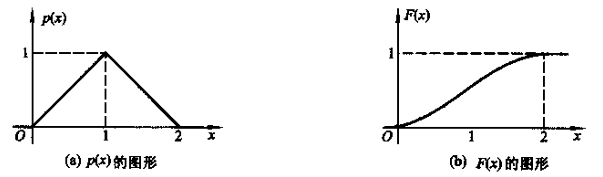
\includegraphics[width=0.7\linewidth]{2-1-7}
	\caption{辛普森分布}
	\label{fig:2-1-7}
\end{figure}

以下我们对密度函数与分布列的异同点作一些说明.

在离散随机变量场合,

\[ 
P(a<X \leqslant b)=\sum_{a<x_{i} \leqslant b} p\left(x_{i}\right)
\]

其中诸$ x_i $;为$ X $的可能取值.

而在连续随机变量场合,

\[ 
P(a<X \leqslant b)=\int_{a}^{b} p(x) \mathrm{d} x
\]

其含义见下图.



\begin{figure}
	\centering
	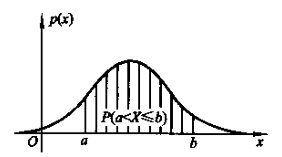
\includegraphics[width=0.7\linewidth]{2-1-8}
	\caption{}
	\label{fig:2-1-8}
\end{figure}

从这个意义上讲,概率密度函数与概率分布列所起的作用是类似的,但它们之间的差别也是明显的,具体有

\begin{enumerate}
	\item 离散随机变量的分布函数F(x)总是右连续的阶梯函数,而连续随机变量的分布函数$ F(x) $一定是整个数轴上的连续函数,因为对任意点$ x $的增量$\Delta x$,相应分布函数的增量总有
	\[ 
	F(x+\Delta x)-F(x)=\int_{x}^{x+\Delta x} p(x) \mathrm{d} x \longrightarrow 0, \quad(\Delta x \rightarrow 0)
	\]
	\item 离散随机变量$ X $在其可能取值的点$x_{1}, x_{2}, \cdots, x_{n}, \cdots$上的概率不为$ 0 $,而连续随机变量$ X $在$(-\infty,+\infty)$上任一点$ a $的概率恒为$ 0 $,即
	\[ 
	P(X=a)=\int_{a}^{a} p(x) \mathrm{d} x=0
	\]
	这表明:不可能事件的概率为$ 0 $,但概率为0的事件不一定是不可能事件;类似地,必然事件的概率为$ 1 $,但概率为$ 1 $的事件不一定是必然事件.
	\item 由于连续随机变量$ X $仅取一点的概率恒为$ 0 $,从而在事件“$a \leqslant X \leqslant b$”
	中减去$ x=a $或减去$ X=b $,不影响其概率,即
	\[ 
	P(a \leqslant x \leqslant b)=P(a<X \leqslant b)=P(a \leqslant X<b)=P(a<X<b)
	\]
	这给计算带来很大方便.而这个性质在离散随机变量场合是不存在的,在离散随机变量场合计算概率要“点点计较”.
	\item 由于在若干点上改变密度函数$ p(x) $的值并不影响其积分的值,从而不影响其分布函数$ F(x) $的值,这意味着一个连续分布的密度函数不唯一.譬如在例2.1.7中,改变$ x=-1 $和x=1处$ p(x) $的值如下:
	\[ 
	p_{1}(x)=\left\{\begin{array}{ll}{0.5,} & {-1 \leqslant x \leqslant 1} \\ {0,} & {\text{其它} \text { th }}\end{array}\right. p_{2}(x)=\left\{\begin{array}{ll}{0.5,} & {-1<x<1} \\ {0} & { \neq 4}\end{array}\right.
	\]
	它们都是$ (-1,1) $上均匀分布的密度函数.但仔细考察这两个函数$ p_1(x) $和$ p_2(x) $,可以发现
	\[ 
	P\left(p_{1}(x) \neq p_{2}(x)\right)=P(X=-1)+P(X=1)=0
	\]
	可见这两个函数在概率意义上是无差别的,在此称$ p_1(x) $与$ p_2(x) $是“几乎处处相等”,其含义是:它们不相等处的点组成集合的概率为$ 0 $.这就是概率论与微积分不同之处,也是概率论的魅力之处.
	除了离散分布和连续分布之外,还有既非离散又非连续的分布,见下例.
\end{enumerate}

\begin{example}
	以下的函数$ F(x) $确是一个分布,它的图形如图~\ref{fig:2-1-9}所示.
	\[ 
	F(x)=\left\{\begin{array}{ll}{0,} & {x<0} \\ {\frac{1+x}{2},} & {0 \leqslant x<1} \\ {1,} & {x \geqslant 1}\end{array}\right.
	\]
	
	从图上可以看出:它既不是阶梯函数,又不是连续图~\ref{fig:2-1-9}既非离散、又非函数,所以它既非离散的又非连续的分布.它是新的一连续的分布函数示例类分布,本书将不研究此类分布,只让大家知道山外有山,需要不断学习与研究.
\end{example}

下面我们再给出一些连续随机变量的例子.

\begin{figure}
	\centering
	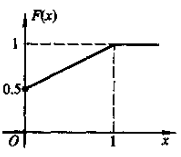
\includegraphics[width=0.7\linewidth]{2-1-9}
	\caption{既非离散、又非连续的分布函数示例}
	\label{fig:2-1-9}
\end{figure}

\begin{example}
	某种型号电子元件的寿命$ X $(以小时计)具有以下的概率密度函数
	\[ 
	p(x)=\left\{\begin{array}{ll}
	\frac{1000}{x^{2}}, &x>1000;\\ 
	{0}, & \text{其它}
	\end{array}\right.
	\]
	现有一大批此种元件(设各元件工作相互独立),问
	
	\begin{enumerate}
		\item 任取1只,其寿命大于1500小时的概率是多少?
		\item 任取4只,4只寿命都大于1500小时的概率是多少?
		\item 任取4只,4只中至少有1只寿命大于1500小时的概率是多少?
		\item 若已知一只元件的寿命大于1500小时,则该元件的寿命大于2000小时的概率是多少?
	\end{enumerate}
\end{example}

\textbf{解}
\begin{enumerate}
	\item \[ 
	P\{X>1500\}=\int_{1500}^{+\infty} \frac{1000}{x^{2}} \mathrm{d} x=\left(-\frac{1000}{x}\right)_{1500}^{+\infty}=\frac{2}{3}
	\]
	\item 各元件工作独立,因此所求概率为
	\[ 
	P\{\text{四只原件寿命都大于}1500\}=[P(X>1500)]^{4}=\left(\frac{2}{3}\right)^{4}=\frac{16}{81}
	\]
	\item 所求概率为
	\[\begin{gathered}
	P\{\text{四只中至少一只寿命大于}1500\} \hfill \\
	=1-P\{4\text{只元件寿命都小于等于}1500\} \hfill \\
	=1-\left(1-\frac{2}{3}\right)^{4}=\frac{80}{81} \hfill \\ 
	\end{gathered} \]
	\item 这是求条件概率$P\{X>2000 | X>1500\}$ ,记
	\[ 
	A=\{X>1500|, B=\{X>2000\}
	\]
	因为$P(A)=2 / 3, P(B)=1 / 2$,且$B \subset A$,所以
	\[ 
	P(B | A)=\frac{P(A B)}{P(A)}=\frac{P(B)}{P(A)}=\frac{3}{4}
	\]
\end{enumerate}

\begin{example}
	向区间$ (0,a) $上任意投点,用X表示这个点的坐标.设这个点落在$ (0,a) $中任一小区间的概率与这个小区间的长度成正比,而与小区间位置无关.求$ X $的分布函数和密度函数.
	
	\textbf{解}
	
	记$ X $的分布函数为$ F(x) $,则
	当$ x<0 $时,因为$\{X \leqslant x\}$是不可能事件,所以$F(x)=P(X \leqslant x)=0$;
	
	当$x \geqslant a$时,因为$\{ X \leqslant x \}$是必然事件,所以$F(x)=P(X \leqslant x)=1$;
	当$0 \leqslant x<a$时,有$F(x)=P(X \leqslant x)=P(0 \leqslant X \leqslant x)=k x$,其中$ k $为比例系数.因为$ 1=F(a)=ka $,所以得$ k=1/a $.
	于是$ X $的分布函数为
	
	\[ 
	F(x)=\left\{\begin{array}{ll}{0,} & {x<0} \\ {\frac{x}{a},} & {0 \leqslant x<a} \\ {1,} & {x \geqslant a}\end{array}\right.
	\]
	
	
	下求$ X $的密度函数$ p(x) $.
	
	当$ x<0 $或$ x>a $时,$ p(x)=F'(x)=0 $;
	
	当$ 0<x<a $时,$ p(x)=F(x)=1/a $;
	
	而在$ x=0 $和$ x=a $处,$ p(x) $可取任意值,一般就近取值为宜,这不会影响概率的计算,因为它们是几乎处处相等的密度函数.于是$ x $的密度函数为
	
	\[ 
	p(x)=\left\{\begin{array}{ll}
	{\frac{1}{a},} & {0<x<a} \\ 
	{0,} & {\text{其它}}
	\end{array}\right.
	\]
	
	这个分布就是区间$ (0,a) $上的均匀分布,记为$ U(0,a) $,其密度函数$ p(x) $
	和分布函数$ F(x) $的图形见下图~\ref{fig:2-1-10}.
\end{example}



\begin{figure}
	\centering
	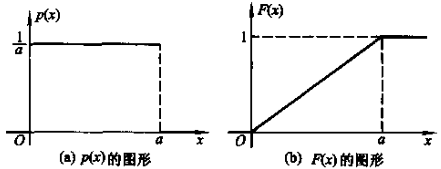
\includegraphics[width=0.7\linewidth]{2-1-10}
	\caption{$ (0,a) $上的均匀分布}
	\label{fig:2-1-10}
\end{figure}

其实此例就是第一章中所说的几何概率,这也建立了几何概率与均匀分布的联系.

\begin{example}
	设连续随机变量X的密度函数为
	
	\[ 
	p(x)=\left\{\begin{array}{ll}
	{4 x^{3},} & {0<x<1}; \\ 
	{0},&{\text{其它}}.
	\end{array}\right.
	\]
	
	(1)已知$ P(X<a)=P(X>a) $,试求常数$ a $(此$ a $称为该分布的中位数).
	
	(2)已知$ P(X>b)=0.05 $,试求常数$ b $.
	
	\textbf{解}
	
	(1) 因为$ X $为连续随机变量,所以有$ P(X=a)=0 $,从而
	\[ 
	P(X<a)+P(X>a)=1
	\]
	
	由$ P(X<a)=P(X>a) $,可以得$ P(X<a)=0.5 $.而
	\[ 
	P(X<a)=\int_{0}^{a} 4 x^{3} d x=a^{4}
	\]
	所以从$ a^4=0.5 $解得$a=\sqrt[4]{0.5}=0.8409$.这里的$ a=0.8409 $把该分布的密度函数下的面积分为两部分,$ a $点左侧与右侧面积各为$ 0.5 $,故称a点为该分布的中位数(详见2.7.4).
	
	(2) 因为
	\[ 
	P(X>b)=\int_{b}^{1} 4 x^{3} \mathrm{d} x=1-b^{4}
	\]
	所以从$1-b^{4}=0.05$解得$b=\sqrt[4]{0.95}=0.9873$.
\end{example}

习题 2.1

1.口袋中有$ 5 $只球,编号为$ 1,2,3,4,5 $.从中任取$ 3 $只,以X表示取出的$ 3 $只球中的最大号码.

(1)试求$ X $的分布列;
(2)写出$ X $的分布函数,并作图.

2.一颗骰子撇两次,以$ X $表示两次中所得的最小点数.

(1)试求$ X $的分布列;

(2)写出X的分布函数.

3.口袋中有$ 7 $个白球、$ 3 $个黑球.

(1)每次从中任取一个不放回,求首次取出白球的取球次数$ X $的概率分布列;

(2)如果取出的是黑球则不放回,而另外放入一个白球,此时$ X $的概率分布列如何.

4.有$ 3 $个盒子,第一个盒子装有1只白球、$ 4 $只黑球;第二个盒子装有$ 2 $只白球、3只黑球;第三个盒子装有$ 3 $只白球、$ 2 $只黑球.现任取一个盒子,从中任取3只球.以$ X $表示所取到的白球数.

(1)试求$ X $的概率分布列;

(2)取到的白球数不少于2只的概率是多少?

5.一批产品共有100件,其中10件是不合格品.根据验收规则,从中任取5件产品进行质量检验,假如5件中无不合格品,则这批产品被接收,否则就要重新对这批产品逐个检验.

(1)试求5件中不合格品数$ X $的分布列;

(2)需要对这批产品进行逐个检验的概率是多少?

6.设随机变量$ X $的分布函数为

\[ 
F(x)=\left\{\begin{array}{ll}
{0,} & {x<0_{i}} \\ {1 / 4,} & {0 \leqslant x<1} \\ 
{1 / 3,} & {1 \leqslant x<3} \\ {1 / 2,} & {3 \leqslant x<6} \\ 
{1,} & {x \geqslant 6}
\end{array}\right.
\]

试求X的概率分布列及$P(X<3), P(X \leqslant 3), P(X>1), P(X \geqslant 1)$.

7.设随机变量X的分布函数为

\[ 
F(x)=\left\{\begin{array}{ll}
{0,} & {x<1} \\ {\ln x,} & {1 \leqslant x<\mathrm{e}_{\mathrm{i}}} \\ 
{1,} & {x \geqslant \mathrm{e}}
\end{array}\right.
\]

试求 $P(X<2), P(0<X \leqslant 3), P(2<X<2.5)$.

8.若$P\left\{X \geqslant x_{1}\right\}=1-\alpha, P\left\{X \leqslant x_{2}\right\}=1-\beta$,其中$ x1<x2 $,试求$P | x_{1} \leqslant X \leqslant x_{2} \}$.

9.从$ 1,2,3,4,5 $五个数中任取三个,按大小排列记为$ x1<x2<x3 $,令$ X=x_2 $,试求

(1)$ X $的分布函数;

(2)$ P(X<2) $及$ P(X>4) $.

10.设随机变量X的密度函数为

\[ 
p(x)=\left\{\begin{array}{ll}
{1-|x|,} & {-1 \leqslant x \leqslant 1} \\ 
{0,} & {\text{其它}}
\end{array}\right.
\]

试求$ P(X≤1.5) $.

12.设随机变量$ X $的密度函数为

\[ 
F(x)=\left\{\begin{array}{ll}
{0,} & {x<0} \\ 
{A x^{2},} & {0 \leqslant x<1} \\ 
{1,} & {x \geqslant 1}
\end{array}\right.
\]

试求

(1)系数$ A $;

(2)$ X $落在区间$ (0.3,0.7) $内的概率;

(3)$ X $的密度函数.

14.学生完成一道作业的时间$ X $是一个随机变量,单位为小时.它的密度函数为

\[ 
p(x)=\left\{\begin{array}{ll}
{c x^{2}+x,} & {0 \leqslant x \leqslant 0.5} \\ 
{0}&{\text{其它}}\end{array}\right.
\]

(1)确定常数$ c $;

(2)写出$ X $的分布函数;
(3)试求在$ 20min $内完成一道作业的概率;

(4)试求$ 10min $以上完成一道作业的概率.

15.设随机变量$ X $和$ Y $同分布,$ X $的密度函数为

\[ 
p(x)=\left\{\begin{array}{ll}
{\frac{3}{8} x^{2},} & {0<x<2} \\ 
{0,} & {\text{其它}}
\end{array}\right.
\]

已知事件$ A=\{X>a——l\} $和$ B=\{Y>a_l\} $独立,且$P(A \cup B)=3 / 4$,求常数$ a $.

16.设连续随机变量X的密度函数$ p(x) $是一个偶函数,$ F(x) $为$ X $的分布函数,求证对任意实数$ a>0 $,有

\[ 
\begin{array}{l}{\text { (1) } F(-a)=1-F(a)=0.5-\int_{0}^{a} p(x) d x_{i}} \\ {\text { (2) } P\left( | X^{*}<a\right)=2 F(a)-1} \\ {\text { (3) } P\left( | X^{\prime}>a\right)=2[1-F(a)]}\end{array}
\]

\subsection{随机变量的数学规堂}

我们已经知道,每个随机变量都有一个分布(分布列、密度函数或分布函数),不同的随机变量可能拥有不同的分布,也可能拥有相同的分布.分布全面地描述了随机变量取值的统计规律性,由分布可以算出有关随机变量事件的概率.除此以外由分布还可以算得相应随机变量的均值、方差、分位数等特征数.这些特征数各从一个侧面描述了分布的特征.譬如,初生婴儿的体重是一个随机变量,其平均重量就是从一个侧面描述了体重的特征.已知随机变量的分布,如何求其均值,是本节需要研究的问题.

本节将介绍随机变量最重要的特征数:数学期望.

\subsection{数学期望的概念}

“期望”在我们日常生活中常指有根据的希望,而在概率论中,数学期望源于历史上一个著名的分赌本问题.
例2.2.1(分赌本问题)17世纪中叶,一位赌徒向法国数学家帕斯卡(1623一1662)提出一个使他苦恼长久的分赌本问题:甲、乙两赌徒赌技相同,各出赌注50法郎,每局中无平局.他们约定,谁先赢三局,则得全部赌本100法郎.当甲赢了二局、乙赢了一局时,因故要中止赌博.现问这100法郎如何分才算公平?

这个问题引起了不少人的兴趣.首先大家都认识到:平均分对甲不公平;全部归甲对乙不公平;合理的分法是,按一定的比例,甲多分些,乙少分些.所以问题的焦点在于:按怎样的比例来分.以下有两种分法:

(1)甲得100法郎中的2/3,乙得100法郎中的1/3.这是基于已赌局数:甲赢了二局、乙赢了一局.

(2)1654年帕斯卡提出如下的分法:设想再赌下去,则甲最终所得X为一个随机变量,其可能取值为0或100.再赌二局必可结束,其结果不外乎以下四种情况之一:

\begin{center}
	甲甲、甲乙、乙甲、乙乙
\end{center}

其中“甲乙”表示第一局甲胜第二局乙胜.因为赌技相同,所以在这四种情况中有三种可使甲获100法郎,只有一种情况(乙乙)下甲获0法郎.所以甲获得100法郎的可能性为$ 3/4 $,获得0法郎的可能性为$ 1/4 $,即$ X $的分布列为

\[ 
\begin{array}{c|cc}{x} & {0} & {100} \\ \midrule
P & {0.25} & {0.75} \\
\end{array}
\]

经上述分析,帕斯卡认为,甲的“期望”所得应为:$0 \times 0.25+100 \times 0.75=75$
(法郎).即甲得75法郎,乙得25法郎.这种分法不仅考虑了已赌局数,而且还包括了对再赌下去的一种“期望”,它比(1)的分法更为合理.

这就是数学期望这个名称的由来,其实这个名称称为“均值”更形象易懂.对上例而言,也就是再赌下去的话,甲“平均”可以赢75法郎.

现在我们来逐步分析如何由分布来求“均值”.

(1)算术平均:如果有$ n $个数$x_{1}, x_{2}, \cdots, x_{n}$.,那么求这$ n $个数的算术平均是很简单的事,只需将此$ n $个数相加后除n即可.

(2)加权平均:如果这$ n $个数中有相同的,不妨设其中有$ n $;个取值为$x_{i}, i=1,2, \cdots, k$.将其列表为

\[
\begin{array}{c|cccc}
\toprule
\text{取值}    &  x_1     &    x_1     &    \cdots     &   x_k \\\midrule
\text{频数}    &  n_1     &    n_2     &     \cdots    &   n_k \\\midrule
\text{频率}    &  n_1/n   &    n_2/n   &     \cdots    &   n_k/n \\
\bottomrule
\end{array}
\]


则其“均值”应为

\[ 
\frac{1}{n} \sum_{i=1}^{k} n_{\dot{r}} x_{i}=\sum_{i=1}^{k} \frac{n_{i}}{n} x_{i}
\]

其实这个“加权”平均的权数“就是出现数值$ x $;的频率,而频率在$ n $很大时,就稳定在其概率附近.

(3)对于一个离散随机变量$ X $,如果其可能取值为$x_{1}, x_{2}, \cdots, x_{n}$.若将这$ n $个数相加后除$ n $作为“均值”,则肯定是不妥的.其原因在于$ X $取各个值的概率是不同的,概率大的出现的机会就大,则在计算中其权也应该大.而上例分配赌本问题启示我们:用取值的概率作为一种“权数”作加权平均是十分合理的.

经以上分析,我们就可以给出数学期望的定义.

\subsection{数学期望的定义}

\begin{definition}
	设离散随机变量$ X $的分布列为
	
	\[ 
	p\left(x_{i}\right)=P\left(X=x_{i}\right), i=1,2, \cdots, n, \cdots
	\]
	
	如果
	
	\[ 
	\sum_{i=1}^{+\infty}\left|x_{i}\right| p\left(x_{i}\right)<+\infty
	\]
	
	则称
	
	\begin{equation} 
	E(X)=\sum_{i=1}^{+\infty} x_{i} p\left(x_{i}\right) \label{eq:2.2.1}
	\end{equation}
	
	为随机变量$ X $的数学期望,或称为该分布的数学期望,简称期望或均值.若级数$\sum_{k=1}^{+\infty}\left|x_{k}\right| p\left(x_{k}\right)$不收敛,则称$ X $的数学期望不存在.
\end{definition}

以上定义中,要求级数绝对收敛的目的在于使数学期望唯一.因为随机变量的取值可正可负,取值次序可先可后,由无穷级数的理论知道,如果此无穷级数绝对收敛,则可保证其和不受次序变动的影响.由于有限项的和不受次序变动的影响,故其数学期望总是存在的.

连续随机变量数学期望的定义和含义完全类似于离散随机变景场合,只要将分布列$ p(x_i) $改为密度函数、将求和改为求积就可.

\begin{definition}
	设连续随机变量$ X $的密度函数为$ p(x) $.如果
	\[ 
	\int_{-\infty}^{+\infty}|x| p(x) \mathrm{d} x<+\infty
	\]
	则称
	
	\begin{equation} 
	E(X)=\int_{-\infty}^{+\infty} x p(x) \mathrm{d} x \label{eq:2.2.2}
	\end{equation}
	为$ X $的数学期望,或称为该分布$ p(x) $的数学期望,简称期望或均值.若$\int_{-\infty}^{+\infty}|x| p(x) \mathrm{d} x$不收敛,则称$ X $的数学期望不存在.
	
\end{definition}

\begin{example}
	在一个人数为$ N $的人群中普查某种疾病,为此要抽验$ N $个人的血.如果将每个人的血分别检验,则共需检验$ N $次.为了能减少工作量,一位统计学家提出一种方法:按$ k $个人一组进行分组,把同组$ k $个人的血样混合后检验,如果这混合血样呈阴性反应,就说明此$ k $个人的血都呈阴性反应,此$ k $个人都无此疾病,因而这$ k $个人只要检验1次就够了,相当于每个人检验$ 1/k $次,检验的工作量明显减少了.如果这混合血样呈阳性反应,就说明此$ k $个人中至少有一人的血呈阳性反应,则再对此$ k $个人的血样分别进行检验,因而这$ k $个人的血要检验$ 1+k $次,相当于每个人检验$ 1+1/k $次,这时增加了检验次数.假设该疾病的发病率为$ p $,且得此疾病相互独立.试问此种方法能否减少平均检验次数?
	
	\textbf{解}
	
	令$ X $为该人群中每个人需要的验血次数,则$ X $的分布列为
	
	\begin{table}[htbp]
		\centering
		\begin{tabular}{c|cc}
			$ x $	&    $ 1 / k $      &  $ 1+1 / k $ \\\midrule
			$ P $	&    $ (1-p)^{k} $  &  $ 1-(1-p)^{k} $\\
		\end{tabular}%
	\end{table}%
	
\end{example}

所以每人平均验血次数为

\[ 
E(X)=\frac{1}{k}(1-p)^{k}+\left(1+\frac{1}{k}\right)\left[1-(1-p)^{k}\right]=1-(1-p)^{k}+\frac{1}{k}
\]

去由此可知,只要选择$ k $使

\[ 
1-(1-p)^{k}+\frac{1}{k}<1, \text{或} \quad(1-p)^{k}>\frac{1}{k}
\]

,就可减少验血次数,而且还可适当选择$ k $使其达到最小.譬如,当$ p=0.1 $时对不同的$ k $,$ E(X) $的值如表~\ref{tab:2.21}所示.从表中可以看出:当$k \geqslant 34$时,平均验血次数超过1,即比分别检验增加工作量;而当$k \leqslant 33$时,平均验血次数在不同程度上得到了减少,特别在$k_{0}=4$时,平均验血次数最少,验血工作量可减少$ 40\% $.

% Table generated by Excel2LaTeX from sheet '1'
\begin{table}[htbp]
	\centering
	\caption{$ p=0.1 $时的$ E(X) $值}
	\begin{tabular}{c|ccccccccc}
		\toprule
		k     & 2     & 3     & 4     & 5     & 8     & 10    & 30    & 33    & 34 \\\midrule
		E(x)  & 0.69  & 0.604 & 0.594 & 0.61  & 0.695 & 0.751 & 0.991 & 0.994 & 1.0016 \\\bottomrule
	\end{tabular}%
	\label{tab:2.21}%
\end{table}%


我们也可以对不同的发病率$ p $计算出最佳的分组人数$ k_0 $,见下表~\ref{tab:2.2.2}.从表中也可以看出:发病率$ p $越小,则分组检验的效益越大.譬如在$ p=0.01 $时,若取11人为一组进行验血,则验血工作量可减少$ 80\% $左右.这正是美国二战期间大量征兵时,对新兵验血所采用的减少工作量的措施.

% Table generated by Excel2LaTeX from sheet '1'
\begin{table}[htbp]
	\centering
	\caption{不同发病率$ p $时的最佳分组人数$ k_0 $及其$ E(x) $}
	\begin{tabular}{c|ccccccc}
		\toprule
		$ p $     & 0.14  & 0.1   & 0.08  & 0.06  & 0.04  & 0.02  & 0.01 \\\midrule
		$ k_0 $    & 3     & 4     & 4     & 5     & 6     & 8     & 11 \\\midrule
		$ E(x) $  & 0.697 & 0.594 & 0.534 & 0.466 & 0.384 & 0.274 & 0.205 \\\bottomrule
	\end{tabular}%
	\label{tab:2.2.2}%
\end{table}%

\begin{example}
	每张福利彩票售价5元,各有一个对奖号.每售出100万张设一个开奖组,用摇奖器当众摇出一个6位数的中奖号码(可以认为从000000到999999的每个数都等可能出现),对奖规则如下:
	\begin{enumerate}
		\item 对奖号与中奖号码的最后一位相同者获六等奖,奖金10元.
		\item 对奖号与中奖号码的最后二位相同者获五等奖,奖金50元.
		\item 对奖号与中奖号码的最后三位相同者获四等奖,奖金500元.
		\item 对奖号与中奖号码的最后四位相同者获三等奖,奖金5000元.
		\item 对奖号与中奖号码的最后五位相同者获二等奖,奖金50000元.
		\item 对奖号与中奖号码的全部相同者获一等奖,奖金500000元.另外规定,只领取其中最高额的奖金.试求每张彩票的平均所得奖金额.
	\end{enumerate}
	
	\textbf{解} 以$ X $记一张彩票的奖金额,则$ X $的分布列如下:
	\[
	\begin{array}{c|ccccccc}
	\toprule
	X     & 500000 & 50000 & 5000  & 500   & 50    & 10    & 0 \\\midrule
	P     & 0.000001 & 0.00009 & 0.00009 & 0.0009 & 0.009 & 0.09  & 0.9 \\\bottomrule
	\end{array}
	\]
	
	
	所以每张彩票的平均所得为
	
	\[ 
	E(X)=0.5+0.45+0.45+0.45+0.45+0.9+0=3.2
	\]
	
	这也意味:每一开奖组把筹得的500万元中的320万元以奖金形式返回给彩民,其余180万元则可用于福利事业及管理费用。
	
	从这个例子也可以看出,彩票中奖与否是随机的,但一种彩票的平均所得是可以预先算出的,计算平均所得也是设计一种彩票的基础.
	
\end{example}

\begin{example}
	设$ x $服从区间$ (a,b) $上的均匀分布,求$ E(x) $.
	
	\textbf{解} 由例2.1.11知$ X $的密度函数为
	
	\[ 
	p(x)=\left\{\begin{array}{ll}
	{\frac{1}{b-a}, }&{a<x<b} \\ {0,}&{\text{其它}}
	\end{array}\right.
	\]
	
	所以
	
	\[ 
	E(X)=\int_{a}^{b} x \cdot \frac{1}{b-a} d x=\frac{1}{b-a} \cdot\left.\frac{x^{2}}{2}\right|_{a} ^{b}=\frac{a+b}{2}
	\]
	
	这个结果是可以理解的,因为X在区间$ (a,b) $上的取值是均匀的,所以它的平均取值当然应该是$ (a,b) $的“中点”,即$ (a+b)/2 $.
	
	
\end{example}

\begin{example}
	柯西分布的数学期望不存在.因为柯西分布的密度函数为
	
	\[ 
	p(x)=\frac{1}{\pi} \frac{1}{1+x^{2}},-\infty<x<+\infty
	\]
	
	所以由
	
	\[ 
	\int_{-\infty}^{+\infty}|x| \cdot \frac{1}{\pi} \frac{1}{1+x^{2}} \mathrm{d} x=+\infty
	\]
	
	知$ E(X) $不存在.
	
\end{example}

\subsection{数学期望的性质}

按照随机变量X的数学期望$ E(X) $的定义,$ E(X) $由其分布唯一确定.如今
若要求随机变量x的一个函数$ g(X) $的数学期望,当然要先求出$ Y=g(X) $的分布,再用此分布来求$ E(Y )$.这一过程可用下面例子说明.

\begin{example}
	已知随机变量$ X $的分布列如下
	
	\[
	\begin{array}{c|ccccc}
	X &{-2} & {-1} & {0} & {1} & {2} \\ \midrule
	P & {0.2} & {0.1} & {0.1} & {0.3} & {0.3}
	\end{array}
	\]
	
	要求$ Y=X^2 $的数学期望,为此要分两步进行:
	
	第一步,先求$ Y=X^2 $的分布,这可从$ X $的分布导出,即
	
	\[
	\begin{array}{c|ccccc}
	X^2    & (-2)^2 & (-1)^2 & 0^2    & 1^2    & 2^2 \\\midrule
	P     & 0.2   & 0.1   & 0.1   & 0.3   & 0.3 \\
	\end{array}
	\]
	
	然后对相等的值进行合并,并把对应的概率相加,可得
	
	\[
	\begin{array}{c|ccc}
	X^2    & 0     & 1     & 4 \\\midrule
	P     & 0.1   & 0.4   & 0.5 \\
	\end{array}
	\]
	
	第二步,利用$ X^2 $的分布求$ E(X^2) $,即得
	
	\[
	E\left(X^{2}\right)=0 \times 0.1+1 \times 0.4+4 \times 0.5=2.4
	\]
	
	假如我们用等值合并前的分布求$ E(X^2) $,可得相同的结果
	
	\[
	E\left(X^{2}\right)=(-2)^{2} \times 0.2+(-1)^{2} \times 0.1+0^{2} \times 0.1+1^{2} \times 0.3+2^{2} \times 0.3=2.4
	\]
	
	这两种算法本质上是一回事,但后者的计算实质上是在$ X $的分布$ (0.2,
	0.1,0.1,0.3,0.3) $基础上、而将取值改为$\left((-2)^{2},(-1)^{2}, 0^{2}, 1^{2}, 2^{2}\right)$计算出来的.由此启发我们:若进一步要求$ E(X^3) $和$ E(X^4) $,我们不需要先求$ X^3 $的分布和$ E\left(X^{4}\right) $的分布,而直接用$ X $的分布来求,具体如下。
	
	\[
	\begin{aligned} 
	E\left(X^{3}\right) &=(-2)^{3} \times 0.2+(-1)^{3} \times 0.1+0^{3} \times 0.1+1^{3} \times 0.3+2^{3} \times 0.3=0 \\ E\left(X^{4}\right) &=(-2)^{4} \times 0.2+(-1)^{4} \times 0.1+0^{4} \times 0.1+1^{4} \times 0.3+2^{4} \times 0.3=8.4 
	\end{aligned}
	\]
	
\end{example}



一般场合,有如下定理:
\begin{theorem}
	若随机变量$ X $的分布用分布列$ p(x_i) $或用密度函数$ p(x) $表示,则$ X $的某一函数$ g(X) $的数学期望为
	
	\begin{equation}
	E[g(X)]=\left\{\begin{array}{ll}
	{\sum_{i} g\left(x_{i}\right) p\left(x_{i}\right)}&{\text{在离散场合;}} \\ {\int_{-\infty}^{+\infty} g(x) p(x) \mathrm{d} x} &{\text{在连续场合.}} 
	\end{array}\right. \label{eq:2.2.3}
	\end{equation}
	
	这里所涉及的数学期望都假设存在.
	
	这个定理的证明涉及更多的工具,在此省略了.现基于这个定理来证明数学期望的几个常用性质,以下均假定所涉及的数学期望是存在的。
	
\end{theorem}

\begin{property}
	
	若$ c $是常数,则$ E(c)=c $.
	
\end{property}

\begin{proof}
	如果将常数$ c $看作仅取一个值的随机变量$ X $,则有$ P(X=c)=1 $,从而其数学期望 $ E(c)=E(X)=c \times 1=c $.
\end{proof}

\begin{property}
	对任意常数$ a $,有
	
	\begin{equation}
	E ( a X ) = a E ( X ) \label{eq:2.2.4}
	\end{equation}
	
\end{property}

\begin{proof}
	在~\ref{eq:2.2.3}式中令$ g(x)=ax $,然后把$ a $从求和号或积分号中提出来即得.
\end{proof}

\begin{property}
	对任意的两个函数$ g_1(x) $和$ g_2(x) $,有
	
	\begin{equation}
	E \left[ g _ { 1 } ( X ) \pm g _ { 2 } ( X ) \right] = E \left[ g _ { 1 } ( X ) \right] \pm E \left[ g _ { 2 } ( X ) \right] \label{eq:2.2.5}
	\end{equation}
	
\end{property}

\begin{proof}
	在~\ref{eq:2.2.3}式中令$ g ( x ) = g _ { 1 } ( x ) \pm g _ { 2 } ( x ) $,然后把和式分解成两个和式,或把积分分解成两个积分即得.
\end{proof}

\begin{example}
	某公司经销某种原料,根据历史资料表明:这种原料的市场需求量X(单位:吨)服从$ (300,500) $上的均匀分布.每售出1吨该原料,公司可获利1.5(千元);若积压1吨,则公司损失0.5(千元).问公司应该组织多少货源,可使平均收益最大?
	
	\textbf{解} 设公司组织该货源$ a $吨.则显然应该有$ 300\leqslant a \leqslant 500 $.又记Y为在$ a $吨货源的条件下的收益额(单位:千元),则收益额$ Y $为需求量$ X $的函数,即$ Y=g(X) $.由题设条件知:当$x \geqslant a$时,则此 $ a $ 吨货源全部售出,共获利$ 1.5a $.当$ X<a $时,则售出$ X $吨(获利$ 1.5X $),且还有$ a-X $吨积压(获利$ -0.5(a-x) $),所以共获利$1.5 X - 0.5 ( a - X )$,由此知
	
	\[
	g ( X ) = \left\{ \begin{array} {ll}
	{ 1.5 a , } & {\text{若}  X \geqslant a } \\ 
	{ 1.5 X - 0.5 ( a - X ) , } & {\text{若}  x < a } 
	\end{array} \right.
	\]
	\[
	\hspace{-0.5ex}=\left\{\begin{array}{ll}
	{1.5 a,} & {\text{若}   X \geqslant a} \\ 
	{2 X-0.5 a,} & {\text{若}   X<a}
	\end{array}\right.
	\]
	
	由定理2.2.1得
	
	\[
	\begin{aligned} E(Y) &=\int_{-\infty}^{+\infty} g(x) p_{X}(x) \mathrm{d} x=\int_{300}^{500} g(x) \frac{1}{200} \mathrm{d} x \\ &=\frac{1}{200}\left\{\int_{a}^{500} 1.5 a \mathrm{d} x+\int_{300}^{a}(2 x-0.5 a) \mathrm{d} x\right\} \\ &=\frac{1}{200}\left(-a^{2}+900 a-300^{2}\right) \end{aligned}
	\]
	
	上述计算表明$ E(Y) $是$ a $的二次函数,用通常求极值的方法可以求得,当$ a
	=450 $吨时,能使$ E(Y) $达到最大,即公司应该组织货源450吨.
	
\end{example}

\begin{center}
	\textbf{习题2.2}
\end{center}

1.设离散型随机变量X的分布列为

\[
\begin{array}{c|ccc}
X & {-2} & {0} & {2} \\ \midrule 
P & {0.4} & {0.3} & {0.3} \\ 
\end{array}
\]

试求$ E(X) $和$ E(3X+5) $.

2.某服装店根据历年销售资料得知:一位顾客在商店中购买服装的件数$ X $的分布列为

\[
\begin{array}{c|cccccc}
X & {0} & {1} & {2} & {3} & {4} & {5} \\ \midrule
P & {0.10} & {0.33} & {0.31} & {0.13} & {0.09} & {0.04}
\end{array}
\]

试求顾客在商店平均购买服装件数.

3.某地区一个月内发生重大交通事故数X服从如下分布
\[
\begin{array}{c|ccccccc}
X     & 0     & 1     & 2     & 3     & 4     & 5     & 6 \\\midrule
P     & 0.301 & 0.362 & 0.216 & 0.087 & 0.026 & 0.006 & 0.002 \\
\end{array}
\]


试求该地区发生重大交通事故的月平均数.

4.一海运货船的甲板上放着20个装有化学原料的圆桶,现已知其中有5桶被海水污染了.若从中随机抽取8桶,记X为8桶中被污染的桶数,试求$ X $的分布列,并求$ E(X) $.

5.用天平称某种物品的重量(砝码仅允许放在一个盘中),现有三组砝码:(甲)$ 1,2,2,5,
10(g $);(乙)$ 1,2,3,4,10(g) $;(两$ )1,1,2,5,10(g) $,称重时只能使用一组砝码,问:当物品的重量为 $1 \mathrm{g}_{1} 2 \mathrm{g}, \cdots, 10 \mathrm{g}$ 的概率是相同的,用哪一组砝码称重所用的平均砝码数最少?

6.假设有十只同种电器元件,其中有两只不合格品、装配仪器时,从这批元件中任取一只,如是不合格品,则扔掉重新任取一只;如仍是不合格品,则扔掉再取一只,试求在取到合格品之前,已取出的不合格品只数的数学期望.

7.对一批产品进行检查,如查到第$ a $件全为合格品,就认为这批产品合格;若在前$ a $件中发现不合格品即停止检查,且认为这批产品不合格.设产品的数量很大,可认为每次查到不合格品的概率都是$ p $.问每批产品平均要查多少件?

8.某厂推土机发生故障后的维修时间$ T $是一个随机变量,其密度函数为

\[
p(t)=\left\{\begin{array}{ll}
{0.02 \mathrm{e}^{-0.02 t},} & {t>0} \\ 
{0,} & {t \leqslant 0}
\end{array}\right.
\]

试求平均维修时间.

9.某新产品在未来市场上的占有率X是仪在区间$ (0,1) $上取值的随机变量,它的密度函数为

\[
p(x)=\left\{\begin{array}{ll}
{4(1-x)^{3},} & {0<x<1;} \\ {0} & {\text{其它.}}
\end{array}\right.
\]

试求平均市场占有率.

10.设随机变量X的密度函数如下,试求$ E(2X+5) $.

\[
p(x)=\left\{\begin{array}{ll}
{\mathrm{e}^{-x},} & {x>0} \\ 
{0,} & {x \leqslant 0}
\end{array}\right.
\]

11.设随机变量$ X $的分布函数如下,试求$ E(X) $.

\[
F(x)=\left\{\begin{array}{ll}
{\frac{e^{x}}{2},} & {x<0} \\ {\frac{1}{2},} & {0 \leqslant x<1} \\
{1-\frac{1}{2} e^{-\frac{1}{2}(x-1)},} & {x \geqslant 1}
\end{array}\right.
\]

12.某工程队完成某项工程的时间$ X $(单位:月)是一个随机变量,它的分布列为

\[
\begin{array}{c|cccc}
X     & 10    & 11    & 12    & 13 \\\midrule
P     & 0.4   & 0.3   & 0.2   & 0.1 \\
\end{array}
\]

(1)试求该工程队完成此项工程的平均月数;
(2)设该工程队所获利润为$ Y=50(13-X) $,单位为万元.试求工程队的平均利润;
(3)若该工程队调整安排,完成该项工程的时间$ X $(单位:月)的分布为

\[
\begin{array}{c|ccc}
{x} & {10} & {11} & {12} \\ \midrule
P & {0.5} & {0.4} & {0.1} \\
\end{array}
\]

则其平均利润可增加多少?

13.设随机变量X的概率密度函数为

\[
p(x)=\left\{\begin{array}{ll}
{\frac{1}{2} \cos \frac{x}{2},} & {0 \leqslant x \leqslant \pi} \\
{0,} & {\text{其它}}
\end{array}\right.
\]

试求 $\frac{1}{x^{2}}$ 的数学期望。

15.设$ X $为仅取非负整数的离散随机变量,若其数学期望存在,证明

\[
E(X)=\int_{0}^{+\infty}[1-F(x)] \mathrm{d} x-\int_{-\infty}^{0} F(x) \mathrm{d} x
\]

\section{随机变量的方是与标准差}


随机变量$ X $的数学期望$ E(X) $是一种位置特征数,它刻画了$ X $的取值总在$ E(X $)周围波动.但这个位置特征数无法反映出随机变量取值的“波动”大小,譬如X与Y的分布列分别为

\[
\begin{array}{c|ccccc|ccc}
X     & -1    & 0     & 1     &       & Y     & -10   & 0     & 10 \\
\cmidrule{1-4}\cmidrule{6-9}    P     & 1/3   & 1/3   & 1/3   &       & P     & 1/3   & 1/3   & 1/3 \\
\end{array}\]

尽管它们的数学期望都是0,但显然$ Y $取值的波动要比X取值的波动大.如何用数值来反映出随机变量取值的“波动”大小,是本节要研究的问题.而以下定义的方差与标准差正是度量此种波动大小的最重要的两个特征数.

\subsection{方整与标准差的定义}

设随机变量X的均值为$ a=E(X) $,$ X $的取值当然不一定恰好是$ a $,会有偏离.偏离的量$ X-a $有正有负,为了不使正负偏离彼此抵消,我们一般考虑$ (X-a)^2 $,而不去考虑数学上难以处理的绝对值$ |X-a| $.因为$ (X-a)^2 $仍是一个随机变量,所以取其均值$ E(X-a)^2 $就可以作为刻画X的“波动”程度,这个量被称作$ X $的方差,其定义如下.
\begin{definition}
	若随机变量$ X^2 $的数学期望$ E(X^2) $存在,则称偏差平方$ (X-EX)^2 $的数学期望$ E(X-EX)^2 $为随机变量$ X $(或相应分布)的方差,记为
	
	\begin{equation}
	\operatorname{Var}(X)=E(X-E(X))^{2}=\left\{\begin{array}{ll}
	{\sum_{i}\left(x_{i}-E(X)\right)^{2} p\left(x_{i}\right)} &{\text{在离散场合;}}\\
	{\int_{-\infty}^{+\infty}(x-E(X))^{2} p(x) \mathrm{d} x} &{\text{在连续场合.}}
	\end{array}\right. \label{eq:2.3.1}
	\end{equation}
	
	称方差的正平方根$\sqrt{\operatorname{Var}(X)}$为随机变量$ X $(或相应分布)的标准差,记为$\boldsymbol{\sigma}(X)$,或$\sigma_X$.
\end{definition}



方差与标准差的功能相似,它们都是用来描述随机变量取值的集中与分散程度(即散布大小)的两个特征数.方差与标准差愈小,随机变量的取值愈集中;方差与标准差愈大,随机变量的取值愈分散.

方差与标准差之间的差别主要在量纲上,由于标准差与所讨论的随机变量、数学期望有相同的量纲,所以在实际中,人们比较乐意选用标准差,但标准差的计算必须通过方差才能算得.
另外要指出的是:如果随机变量X的数学期望存在,其方差不一定存在;而当$ X $的方差存在时,则$ E(X) $必定存在,其原因在于 $|x| \leqslant x^{2}+1$ 总是成立的.

\begin{example}
	图~\ref{fig:2-3-1}上有三个分布:三角分布、均匀分布和倒三角分布的密度函数及它们的图形.从图上可以看出,这三个分布都位于区间(-1,1)上,并且关于纵轴对称,从而得知这三个分布的期望均为0.但它们的方差不等(因此标准差也不等),这可分别由各自的分布算得
	
	\[
	\begin{aligned}
	\operatorname{Var}\left(X_{1}\right)&=E\left(X_{1}^{2}\right)=\int_{-1}^{\theta} x^{2}(1+x) \mathrm{d} x+\int_{0}^{1} x^{2}(1-x) \mathrm{d} x=\frac{1}{6}\\
	\operatorname{Var}\left(X_{2}\right) &=E\left(X_{2}^{2}\right)=\int_{-1}^{1} \frac{x^{2}}{2} \mathrm{d} x=\frac{1}{3} \\ 
	\operatorname{Var}\left(X_{3}\right) &=E\left(X_{3}^{2}\right)=\int_{-1}^{0} x^{2}(-x) \mathrm{d} x+\int_{0}^{1} x^{2} \cdot x \mathrm{d} x=\frac{1}{2} 
	\end{aligned}
	\]
	
	这些计算结果与我们直观对分布的认识是一致的.在这三个分布中,三角分布在中间较为集中,故方差最小;而倒三角分布集中于两侧,故方差最大;均匀分布介于其中,故方差也介于其中.我们将三个分布的数学期望、方差和标准差都列于图2.3.1的相应分布的右侧,以供比较.
	
\end{example}


\begin{figure}[h!]
	\begin{minipage}{0.3\textwidth}
		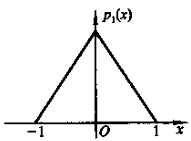
\includegraphics[width=0.7\linewidth]{2-3-1-a}
		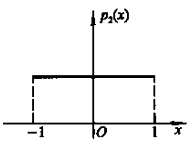
\includegraphics[width=0.7\linewidth]{2-3-1-b}
		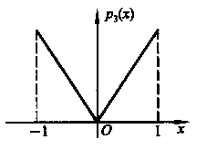
\includegraphics[width=0.7\linewidth]{2-3-1-c}
	\end{minipage}
	\begin{minipage}{0.3\textwidth}
		
		\[
		p_{1}(x)=\left\{\begin{array}{ll}
		{1+x,} & {-1 \leqslant x<0 ;} \\ 
		{1-x,} & {0 \leqslant x<1 ;} \\ 
		{0}    & {\text{其它.}}
		\end{array}\right.
		\]
		
		\[
		p_{2}(x)=\left\{\begin{array}{ll}
		{1 / 2,} & {-1<x<1 ;} \\ 
		{0,}     & {\text{其它.}}
		\end{array}\right.
		\]
		
		\[
		p_{3}(x)=\left\{\begin{array}{ll}
		{-x,} & {-1 \leqslant x<0 ;} \\ 
		{x,}  & {0 \leqslant x<1 ;}   \\ 
		{0,}  & {\text{其它.}}
		\end{array}\right.
		\]
		
	\end{minipage}\qquad \quad
	\begin{minipage}{0.3\textwidth}
		
		\vspace{-5ex}
		\begin{center}
			期望 \quad 方差 \quad 标准差
		\end{center}
		
		\vspace*{-2ex}
		
		\[
		{0 \qquad \quad \frac{1}{6} \qquad 0.4082}
		\]
		
		\vspace{3ex}
		
		\[
		{0 \qquad \quad \frac{1}{3} \qquad 0.5774}
		\]
		
		
		\vspace{3ex} 
		
		\[
		{0 \qquad \quad \frac{1}{2} \qquad 0.7071} 
		\]
		
		
	\end{minipage}
	\caption{比较三个分布的方差与标准差}
	\label{fig:2-3-1}
\end{figure}

\begin{example}
	某人有一笔资金,可投入两个项目:房产和商业,其收益都与市场状态有关.若把未来市场划分为好、中、差三个等级,其发生的概率分别为$ 0.2、0.7、0.1 $.通过调查,该投资者认为投资于房产的收益$ X $(万元)和投资于商业的收益$ Y $(万元)的分布分别为
	
	\[
	\begin{array}{c|ccccc|ccc}
	X     & 11    & 3     & -3    &       & Y     & 6     & 4     & -1 \\
	\cmidrule{1-4}\cmidrule{6-9}    P     & 0.2   & 0.7   & 0.1   &       & P     & 0.2   & 0.7   & 0.1 \\
	\end{array}
	\]
	
	请问:该投资者如何投资为好?
	
	\textbf{解} 我们先考察数学期望(平均收益)
	
	\[
	\begin{array}{c}
	{E(X)=11 \times 0.2+3 \times 0.7+(-3) \times 0.1=4.0 (\text{万元})} \\ 
	{E(Y)=6 \times 0.2+4 \times 0.7+(-1) \times 0.1=3.9(\text{万元})}
	\end{array}
	\]
	
	从平均收益看,投资房产收益大,可比投资商业多收益0.1万元.下面我们再来计算它们各自的方差
	
	\[
	\begin{aligned} 
	\operatorname{Var}(X) &=(11-4)^{2} 1 \times 0.2+(3-4)^{2} \times 0.7+(-3-4)^{2} \times 0.1=15.4 \\ 
	& \operatorname{Var}(Y)=(6-3.9)^{2} \times 0.2+(4-3.9)^{2} \times 0.7+(-1-3.9)^{2} \times 0.1=3.29 
	\end{aligned}
	\]
	
	及标准差
	
	\[
	\sigma(X)=\sqrt{15.4}=3.92, \sigma(Y)=\sqrt{3.29}=1.81
	\]
	
	因为标准差(方差也一样)愈大,则收益的波动大,从而风险也大.所以从标准差看,投资房产的风险比投资商业的风险大一倍多.若收益与风险综合权衡,该投资者还是应该选择投资商业为好,虽然平均收益少0.1万元,而风险要小一半以上.
	
\end{example}

\subsection{方整的性质}

以下均假定随机变量的方差是存在的.

\begin{property}
	\[
	\operatorname{Var}(X)=E\left(X^{2}\right)-[E(X)]^{2}
	\]
	
	\begin{proof}
		因为 $ \operatorname{Var}(X)=E(X-E(X))^{2}=E\left(X^{2}-2 X \cdot E(X)+(E(X))^{2}\right)$ , 由数学期望的性质2.2.3可得
		
		\[
		\operatorname{var}(X)=E\left(X^{2}\right)-2 E(X) \cdot E(X)+(E(X))^{2}=E\left(X^{2}\right)-(E(X))^{2}
		\]
		
	\end{proof}	
	
	在实际计算方差时,这个性质往往比定义 $\operatorname{Var}(X)=E(X-E X)^{2}$ 更常用.
	
\end{property}

\begin{property}
	常数的方差为0,即 $\mathrm{Var}(c)=0$ ,其中$ c $是常数.
\end{property}

\begin{proof}
	若$ c $是常数,则
	
	\[
	\operatorname{Var}(c)=E(c-E(c))^{2}=E(c-c)^{2}=0
	\]
	
\end{proof}	


\begin{property}
	若a,b是常数,则 $\operatorname{Var}(a X+b)=a^{2} \operatorname{Var}(X)$ .
\end{property}

\begin{proof}
	若$ a,b $是常数,则
	
	\[
	\begin{aligned} \operatorname{Var}(a X+b) &=E(a X+b-E(a X+b))^{2} \\ &=E(a(X-E(X)))^{2} \\ &=a^{2} \operatorname{Var}(X) \end{aligned}
	\]
	
	另外从 $\operatorname{Var}(X)=E\left(X^{2}\right)-[E(X)]^{2} \geqslant 0$ 很容易看出:若$ E(X^2)=0 $,则$ E(X)=0 $,且 $\operatorname{Var}(X)=0$ .
	
\end{proof}

\begin{example}
	设$ X $为掷一颗骰子出现的点数,试求 $\operatorname{Var}(\boldsymbol{X})$ .
	
	\textbf{解}
	
	\[
	\begin{array}{l}{E(X)=\frac{1}{6}(1+2+3+4+5+6)=\frac{7}{2}} \\ {E\left(X^{2}\right)=\frac{1}{6}\left(1^{2}+2^{2}+3^{2}+4^{2}+5^{2}+6^{2}\right)=\frac{91}{6}} \\ {\operatorname{Var}(X)=\frac{91}{6}-\frac{49}{4}=\frac{35}{12}=2.917}\end{array}
	\]
	
\end{example}

\subsection{切比雪夫不等式}

下面给出概率论中一个重要的基本不等式.

\begin{theorem}
	(切比雪夫$ (1821一1894) $不等式)设随机变量$ X $的数学期望和方差都存在,则对任意常数$ e>0 $,有
	
	\begin{equation}
	P(|X-E X| \geqslant \epsilon) \leqslant \frac{\operatorname{Var}(X)}{\varepsilon^{2}} \label{eq:2.3.2}
	\end{equation}
	或
	\begin{equation}
	P(|X-E X|<\varepsilon) \geqslant 1-\frac{\operatorname{Var}(X)}{\varepsilon^{2}} \label{eq:2.3.3}
	\end{equation}
\end{theorem}

\begin{proof}
	没$ X $是一个连续随机变量,其密度函数为$ p(x) $.记$ E(X)=a $,我们有
	
	\[
	\begin{array}{ll}
	{P(|X-a| \geqslant \varepsilon)} & {=\int_{\{x | x-a \geq \epsilon\}} p(x) \mathrm{d} x \leq \int_{\{x | x-a>c\}} \frac{(x-a)^{2}}{\varepsilon^{2}} p(x) \mathrm{d} x} \\ 
	{} & {\leqslant \frac{1}{\varepsilon^{2}} \int_{-\infty}^{+\infty}(x-a)^{2} p(x) \mathrm{d} x=\frac{\operatorname{Var}(X)}{\varepsilon^{2}}}
	\end{array}
	\] 
\end{proof}

由此知~\ref{eq:2.3.2}式对连续随机变量成立,对于离散随机变量亦可类似进行证明.

在概率论中,事件“ $|X-E(X)| \geqslant \varepsilon$ ”称为大偏差,其概率 $ P(1X-E(X)1 \geqslant e) $ 称为大偏差发生概率.切比雪夫不等式给出大偏差发生概率的上界,这个上界与方差成正比,方差愈大上界也愈大.
以下定理进一步说明了方差为0就意味着随机变量的取值集中在一点上.

\begin{theorem}
	若随机变量$ X $的方差存在,则 $\operatorname{Var}(X)=0$ 的充要条件是$ X $几乎处处为某个常数$ a $,即$ P(X=a)=1 $.
\end{theorem}

\begin{proof}
	充分性是显然的,下面证必要性.设 $\operatorname{Var}(X)=0$ ,这时$ E(X) $存在.因为
	
	\[
	| | X-E(X)|>0|=\bigcup_{n=1}^{+\infty}\left\{|X-E(X)| \geqslant \frac{1}{n}\right\}
	\]
	
	所以有
	
	\[
	\begin{aligned} P(|X-E(X)|>0) &=P\left(\bigcup_{n=1}^{n}\left\{|x-E(X)| \geqslant \frac{1}{n}\right\}\right) \\ & \leqslant \sum_{n=1}^{+\infty} P\left(|X-E(X)| \geqslant \frac{1}{n}\right) \leqslant \sum_{n=1}^{+\infty} \frac{\operatorname{Var}(X)}{(1 / n)^{2}}=0 \end{aligned}
	\]
	
	其中最后一个不等式用到了切比雪夫不等式.由此可知
	
	\[
	P(|X-E(X)|>0)=0
	\]
	
	因而有
	
	\[
	P(|X-E(X)|=0)=1
	\]
	
	即
	
	\[
	P(X=E(X))=1
	\]
	
	这就证明了结论,且其中的常数$ a $就是$ E(X) $.
\end{proof}

\begin{center}
	\textbf{习题2.3}
\end{center}

1.设随机变量$ X $满足$E(X)=\operatorname{Var}(X)=\lambda$,已知$ E[(X-1)(x-2)]=1 $,试求$\lambda$.

2.假设有10只同种电器元件,其中有两只不合格品.装配仪器时,从这批元件中任取一只,如是不合格品,则扔掉重新任取一只;如仍是不合格品,则扔掉再取一只,试求在取到合格品之前,已取出的不合格品只数的方差.

3.已知$ E(X)=-2,E(X2)=5 $,求$(\operatorname{Var}(1-3 X)$.

4.设随机变量$ X $的分布函数为

\[
F(x)=\left\{\begin{array}{ll}{\frac{e^{x}}{2},} & {x<0} \\ {\frac{1}{2},} & {0 \leqslant x<1 \}} \\ {1-\frac{1}{2} \mathrm{e}^{-\frac{1}{2}(x-1)}, x \geqslant 1}\end{array}\right.
\]

试求$\operatorname{Var}(X)$.

5.设随机变量$ X $的密度函数为

\[
p(x)=\left\{\begin{array}{ll}
{1+x,} & {-1<x \leqslant 0 ;} \\ 
{-1<x \leqslant 0 ;} & {0<x \leqslant 1 ;} \\ 
{0} & {\text{其它}}
\end{array}\right.
\]
试求 $\mathrm{Var}(3 X+2)$ 。

6.试证:对任意的常效$ c $关$ E(X) $,有

\[
\operatorname{Var}(X)=E(X-E(X))^{2}<E(X-c)^{2}
\]

7.设随机变量X仅在区间 $[a, b]$ 上取值,试证

\[
a \leqslant E(X) \leqslant b, \operatorname{Var}(X) \leqslant\left(\frac{b-a}{2}\right)^{2}
\]

18.设随机变量$ X $取值x1≤…≤x。的概率分别是 $x_{1} \leqslant \cdots \leqslant x_{n}$ .证明

\[
\operatorname{Var}(X) \leqslant\left(\frac{x_{\mathrm{n}}-x_{1}}{2}\right)^{2}
\]

9.设g(x)为随机变置$ X $取值的集合上的非负不减函数,且$ E(g(X)) $存在,证明:对任意的 $\varepsilon>0$ ,有

\[
P(X>\varepsilon) \leqslant \frac{E(g(X))}{g(\varepsilon)}
\]

10.设$ X $为非负随机变量,$ a>0 $.若 $E\left(\mathrm{e}^{a X}\right)$ 存在,证明:对任意的$ x>0 $,有

\[
P(X \geqslant x) \leqslant \frac{E\left(\mathrm{e}^{a X}\right)}{\mathrm{e}^{a x}}
\]

11.已知正常成人男性每毫升血液中的白细胞数平均是7300,标准差是700.试利用切比雪夫不等式估计每升血液中的白细胞数在5200至9400之间的概率的下界.